\section{Muon System}
Good muon detection and resolution is of central importance 
to the CMS detector due the muon's appearance in the final state of many important processes
(for example H$\rightarrow$ZZ$\rightarrow\mu\mu\mu\mu$ and H$\rightarrow\tau\tau$ 
with $\tau\rightarrow\mu\bar{\nu_{\mu}}\nu_{\tau}$). 
The muon is a relatively easy particle to detect; due to its long lifetime 
and heavy mass it is less affected by radiative losses and the
CMS detector is capable of reconstructing muon momentum and charge over the entire
kinematic range of the LHC. The muon system covers the region in pseudorapidity
$|\eta|<2.4$, consists of about 25,000 m$^{2}$ of 3
 different types of gaseous particle detectors: drift tube (DT) chambers, 
 cathode strip chambers (CSC) and resistive plate chambers (RPCs).
 Their selection and location are determined by the relative occupancy
 of muons in the detector and the uniformity of the magnetic field.
 For example, DTs are more sensitive to a nonuniform magnetic field, therefore,
 they are used only in the CMS barrel. The location of the muon subsystems
 can be seen in Figure \ref{fig:muonLayout}. 
 \begin{figure}[hb]
  \centering
	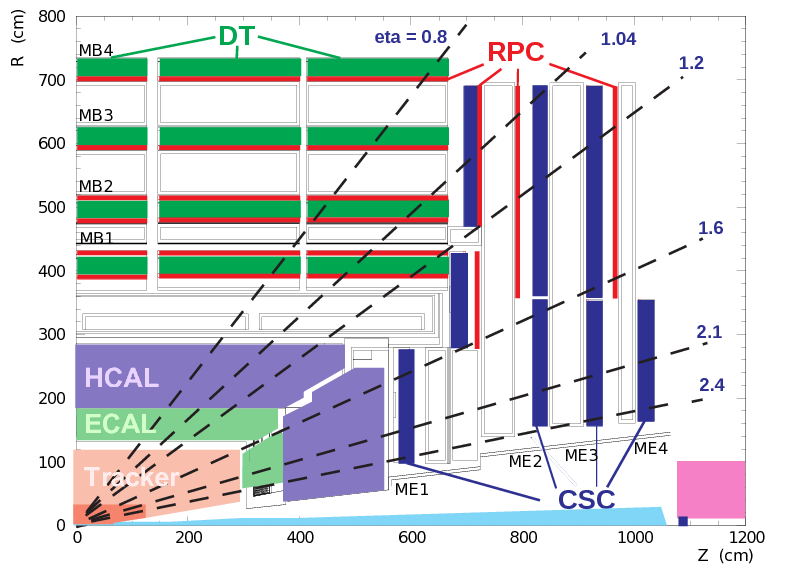
\includegraphics[width=0.75\textwidth]{images/muonSysLayout.png}
  	\caption[Layout of the Muon Sub-Detector]
   	{Detailed view of the placement of muon detectors within the muon system.}
	\label{fig:muonLayout}
\end{figure}
 
\subsection{Drift Tube System}
The barrel region has a low muon rate as well as a low flux of neutrons (which are left over 
from hadronic decays) and a uniform 3.8 T magnetic field. 
Drift tube chambers with standard rectangular drift cells, 
which are more sensitive to these environmental effects but are 
relatively cheaper and easier to produce, are used in this region. 
They cover the pseudorapidity region $|\eta|<1.2$ and are stationed within 
the iron yoke. The barrel muon detector consists of 4 concentric
cylinders of drift tube chambers around the beam line. The 3 inner
cylinders have 60 DT chambers while the outer has 70 DT chambers,
these combine to a total of approximately 172,000 sensitive wires.
\begin{figure}[hb]
  \centering
	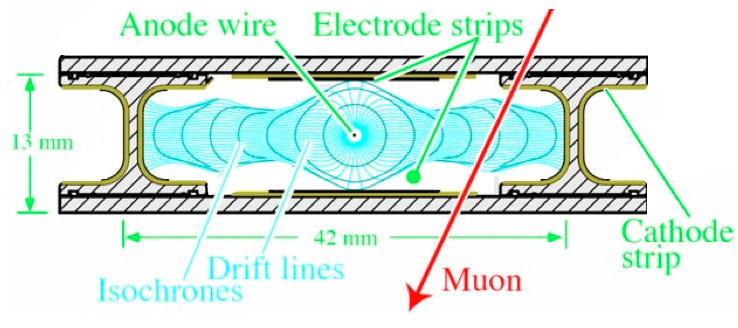
\includegraphics[width=0.75\textwidth]{images/driftCell.png}
  	\caption[Individual Drift Cell]
   	{An Individual Drift Cell of the Drift Tube Chamber System}
	\label{fig:driftCell}
\end{figure}
The DT Chambers are made up of three (or two) super-layers (SL), the 
SL is further divided into individual drift tube cells. 
A diagram of a drift cell is shown in figure \ref{fig:driftCell},
each drift cell contains an anode wire that is 50 $\mu$m in diameter
and two electrode plates that create the drift electric field. The walls
of the cell are grounded, acting as cathodes. Each cell is filled with a gas
mixture of 85\% Argon and 15\% Carbon Dioxide; the wire and the
electrodes are operated with a voltage difference of 1.8 kV. Each
SL is made of four layers of drift cells staggered by half a cell.
The wires of the inner SLs are aligned perpendicular to the beam line
to provide a measurement of the z position of the track while the 
outer SLs have wires aligned parallel to the beam line to 
to provide a measurement in the transverse plane. 

\subsection{Cathode Strip Chambers}
The Cathode Strip Chambers (CSC) are installed in the CMS endcaps.
Due to their granularity and fast signal response time they are able to provide precision muon 
position measurement and a muon trigger signal in one device. CSCs do not 
require precise gas, temperature or pressure control and are also capable of operating
in non-uniform magnetic fields, which make them an ideal candidate for higher
ranges of pseudorapidity. 
\begin{figure}[hb]
  \centering
	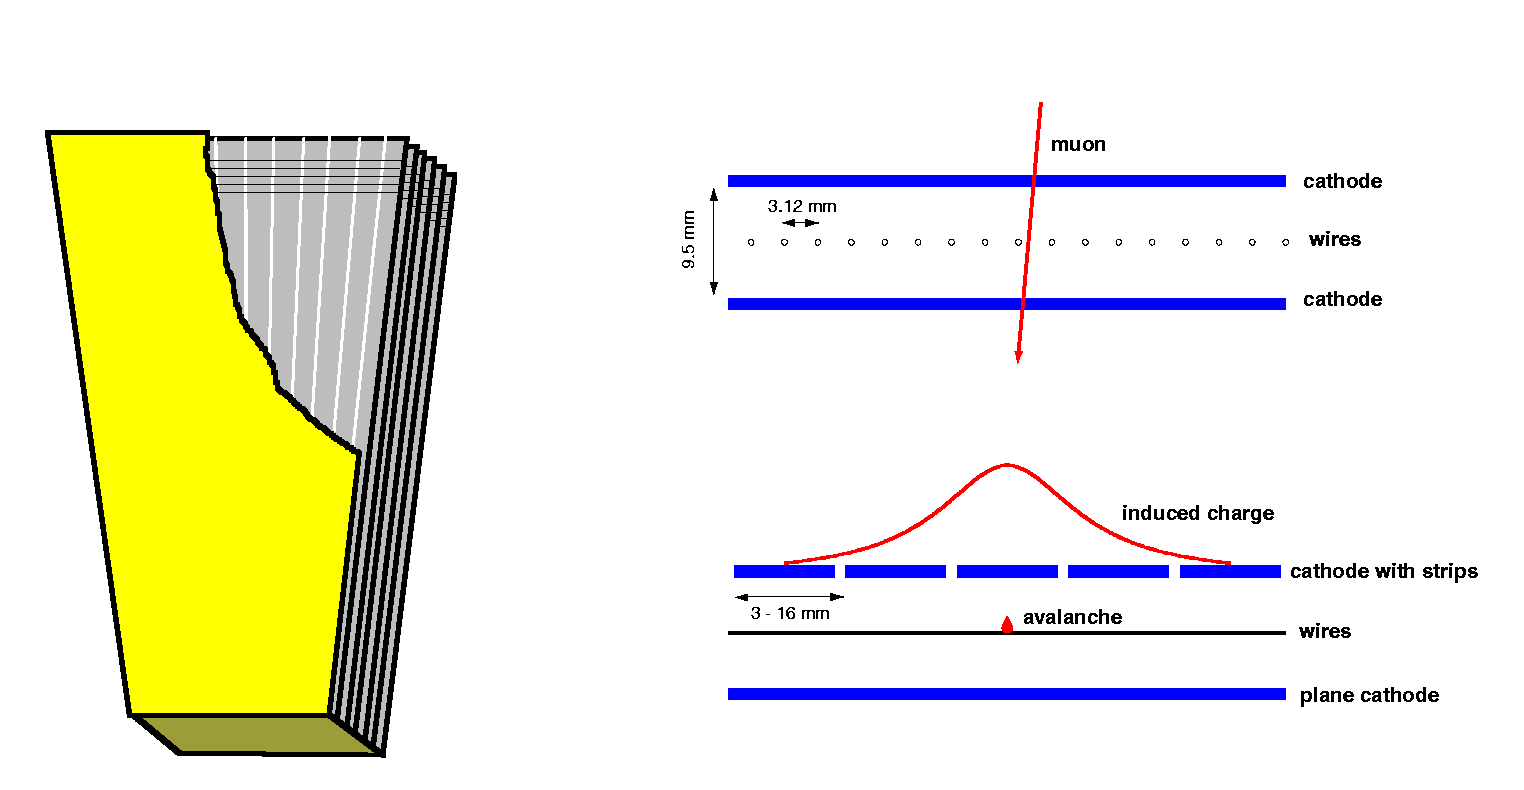
\includegraphics[width=1\textwidth]{images/CSC2images.png}
  	\caption[Cathode Strip Chambers]
   	{Front view of CSC and cross-sectional view of CSC}
	\label{fig:cscImage}
\end{figure}
As is illustrated in Figure \ref{fig:cscImage},
the CSCs consist of 7 trapezoidal panels with cathode strips which are interweaved with
6 planes of anode wires. Wires run azimuthally and define a track's 
radial component. The path of a charged muon is found by interpolating charges
on the cathode strips by the avalanche of positive ions which is catalyzed by
the charged muon; the signal is then generated by dipole moment of the ionized atoms
when electrons are pulled off. %%check this in an alternate source, still confused about how signal is transported, through wire?
Muons from $1.2<|\eta|<2.4$ cross 3 or 4 CSCs. In total the CSC system provides
a combined 5000 m$^2$ of sensitive planes and has over 2 million wires.
The trapezoidal CSCs cover either 10$^{\o}$ or 20$^{\o}$ in $\phi$
%, all chambers their placement in the detector 
 with overlap to form continuous $\phi$ coverage (excluding the ME1/3 ring).
%Muons that traverse the region $0.9<|\eta|<1.2$ are also detected by resistive plate chambers. 

\subsection{Resistive Plate Chambers}
Resistive plate chambers (RPCs) are installed up to $|\eta|<$1.6. 
RPCs are much faster than the 25ns bunch crossing time and, therefore,
are used for triggering as well as muon kinematic measurements. 
As can be seen in Figure \ref{fig:RPCsketch},
\begin{figure}[hb]
  \centering
	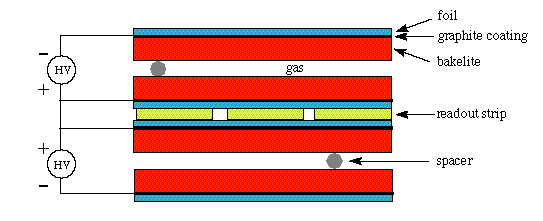
\includegraphics[width=0.9\textwidth]{images/RPCsketch.png}
  	\caption[RPC Sketch]
   	{Layout of a Double Gap RPC}
	\label{fig:RPCsketch}
\end{figure}
RPCs are composed
of two parallel plates which are separated by gas and they are operated in avalanche 
mode with readout strips in between. 
RPCs need intensive monitoring of temperature, humidity and pressure to ensure stability
of conditions for proper operation.
During 2011 and 2012 the CMS detector had six layers of RPC chambers in the barrel iron yoke,
2 located in each of the first and second muon stations and 1 in each of the last stations.
%During Long Shutdown 1 more RPCs were installed in the endcap. 
